\section{Γρφικά Υπολογιστών}
\label{appendix:computer_graphics}


\begin{definition}[Κατακόρυφο διάνυσμα κορυφής]
\label{definition:vertex_normal}
 
 Στη γεωμετρία των γραφικών υπολογιστών, ένα κάθετο διάνυσμα κορυφής (\textsl{vertex normal}) ενός τρισδιάστατου πολύεδρου είναι το ευκλείδιο διάνυσμα κατεύθυνσης στο σημείο, όπως φαίνεται στο Σχήμα \ref{fig:vertex_normal}. Το κάθετο διάνυσμα στην επιφάνεια που σχηματίζουν τα τρίγωνα χρησιμοποιείται στα γραφικά υπολογιστών για τον υπολογισμό της αντανάκλασης του φωτός όπως φαίνεται στο Σχήμα \ref{fig:vertex_normal_reflection}

\begin{figure}[h]
\label{fig:vertex_normal}	
\centering
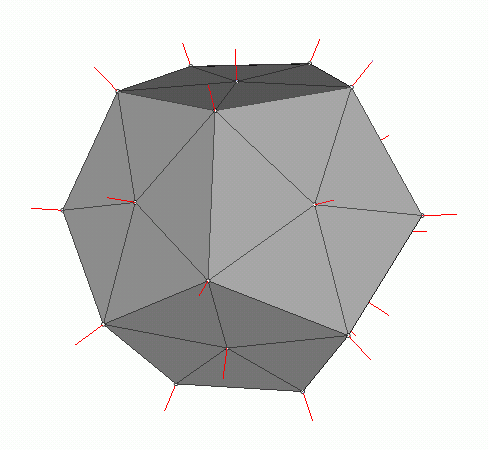
\includegraphics[scale=0.2]{images/appendix/vertex_normal.png}
\caption[Κάθετα διανύσματα κορυφών πολύεδρου]{Τα κάθετα διανύσματα ενός δωδεκάεδρου πλέγματος σε κάθε κορυφή των τριγώνων που το σχηματίζουν.}
\end{figure}

\begin{figure}[h]
\label{fig:vertex_normal_reflection}	
\centering
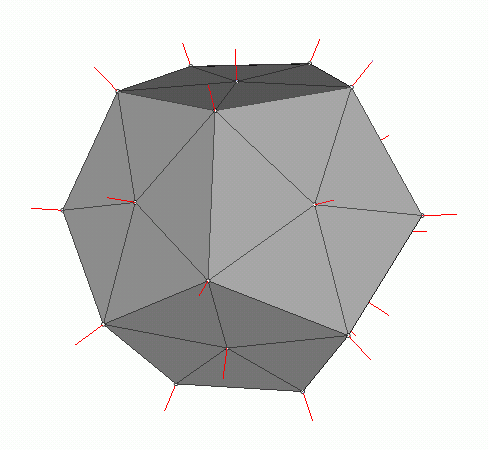
\includegraphics[scale=0.2]{images/appendix/vertex_normal.png}
\caption[Αντανάκλαση του φωτός στο κάθετο διάνυσμα]{Τα κάθετα διανύσματα ενός δωδεκάεδρου πλέγματος σε κάθε κορυφή των τριγώνων που το σχηματίζουν.}
\end{figure}

\end{definition}